% 记录一些常见的图的概念
\subsection{图基本概念}
\paragraph{Motif} 形式上是一个连通子图,强调这个Motif的拓扑结构。Motif可能是某种经常出现在图中的结构,可以认为时一种反复出现的结构模式。相同结点数的motif可能会有多种结构。

\paragraph{Weisfeiler-Lehman isomorphism test}  图同构测试。对于两个图$G_1, G_2$,WL test能够判断它们是否同构,但是也存在一些特殊的例子,WL test会将非同构的两个图判定为同构的。算法过程如下:
\begin{enumerate}
	\item 对$G_1, G_2$中的结点都赋予一个标签,都为1;
	\item 对于每个结点$v$重复执行:
	\begin{enumerate}
		\item 汇集$v$的邻居结点的标签,放在一个列表里,$S_v = \{u_l | u \in \mathcal{N}_v \}$
		\item 将$v$的标签$v_l$和S组合成一个pair---$(v_l, S_v)$
	\end{enumerate}
	\item 利用一个hash函数将每个结点的$(v_l, S_v)$映射成一个新的标签,将新的标签赋予给对应的结点。至此一轮迭代就结束了,如果图中结点的标签都没发生变化则结束,否则返回步骤2.
\end{enumerate}
上述过程是针对一个图来说的,可以同时分别对$G_1, G_2$执行上述算法。
当迭代结束后怎么判定两个图是否同构呢?
WL test中是这样做的:\\
分别计算图中每个标签的数量(也就是标签的分布),可能会得到类似这样的一个结果(1: 2, 2:3, ...),这表示标签1出现了2次,标签2出现了3次。如果最后两个图这个结果是一致的,那么不排除它们同构的可能性。

基于WL test 算法,WL subtree kernel\cite{shervashidze2011weisfeiler} 构建以某个结点为根的子树,来代表该结点的特征。

\paragraph{图算法(GNN)中常用的benchmar以及数据集} 常用的图数据集主要可以分为这几类:
\begin{itemize}
	\item 生物信息类的图数据。如MUTAG, PTC, NCI1,PROTEINS 分子,药物的一些图数据
	\item 社交网络。如Facebook, Reddit 等
	\item 引文网络。如 Cora, PubMed, Citeseer等
\end{itemize}

斯坦福大学的SNAP组有很丰富的图网络数据集:\href{http://snap.stanford.edu/data/index.html}{Stanford Large Network Dataset Collection}


\paragraph{Heterogeneous graph, Attributed graph}同构图和属性图,同构图中,有多种类型的结点和边。Attributed graph中结点会有较丰富的属性(个人感觉可以理解为特征)。一个简单的分类:
\begin{table}[h]
	\centering
	\begin{tabular}{|c|c|c|c|}
		\hline
		\rowcolor[HTML]{4371C3} 
		{\color[HTML]{FFFFFF} \textbf{Graph Types}}                            & {\color[HTML]{FFFFFF} \textbf{Homogeneous}} & {\color[HTML]{FFFFFF} \textbf{Multi-Relational}} & {\color[HTML]{FFFFFF} \textbf{Heterogeneous}} \\ \hline
		\rowcolor[HTML]{CED6EA} 
		\textbf{\#of node types}                                               & \textbf{1}                                  & \textbf{1}                                       & \textbf{\textgreater{}1}                      \\ \hline
		\rowcolor[HTML]{E9EBF6} 
		\multicolumn{1}{|l|}{\cellcolor[HTML]{E9EBF6}\textbf{\#of edge types}} & \textbf{1}                                  & \textbf{\textgreater{}1}                         & \textbf{\textgreater{}=1}                     \\ \hline
	\end{tabular}
\end{table}

\paragraph{Graph Kernel}

\paragraph{Dynamic graph, Streaming graph}动态图和流图。动态图主要指在给定的(static)的结点集上,随着时间,边发生变化;而流图则是结点集和边都会随着时间而变化。

除了结点和边的变化,可能结点/边的标签也会发生变化,更具体的,结点/边的属性也会变化。

\paragraph{图的同构}对于两个图$\mathcal{G}_1 = (V_1, G_2), \mathcal{G}_2=(V_2, E_2)$,如果两图之间的结点能够一一对应,令该映射为$f$,

若$\forall v_i^1, v_j^1 \in V_1, v_i^2, v_j^2 \in V_2$,$f(v_i^1) = v_i^2, f(v_j^1) = v_i^2$,当$(v_i^1, v_j^1) \in E_1$有$( f(v_i^2), f(v_j^2) ) \in E_2$,则称$\mathcal{G}_1, \mathcal{G}_2$是同构的,存在同构映射$f$。

\subsection{结点邻居采样}
在图机器学习中,生成结点表征可以说是最基本的事儿了。不管是随机游走、矩阵分解还是图神经网络的方式,最终都会得到结点的表征。其中不可绕过的一个就是结点的邻居。
在随机游走中,会类似于语言模型中词语的上下文环境一样为结点构造上下文,每个结点产生的随机游走路径就是一个上下文。游走的过程可以看作是对结点邻居进行采样的过程。矩阵分解中,通常是构造图的Laplacian矩阵,再进行分解,用特征向量来表示结点表征,对这个不是很了解,就不多说了。到了图神经网络中,节点邻居更是成了主角。从GCN原论文\cite{kipf2017semi-supervised} ==> GraphSage\cite{hamilton2017inductive} ==> FastGCN\cite{chen2018fastgcn} ==> VR-GCN\cite{chen2018stochastic} ==> ... 。GCN中结点的邻居采样方式五花八门。

\begin{enumerate}
	\item GCN原论文中,再进行图卷积时需要把整个graph全部加载进内存,为了求一个结点的表征需要对整个graph进行卷积
	\item GraphSage中,并不使用结点的所有邻居,而是对每个结点的邻居进行采样,得到固定数目的采样后的邻居
	\item FastGCN中引入了importance sampling
	\item 审稿时发现的根据attention distribution 和 uniform distribution的KL散度选top-k的采样。这种方法可以发现比较重要的结点,而不是均匀地参与到其邻居的结点
\end{enumerate}

\subsection{DeepWalk \& Node2Vec}
二者都是学习结点表征的方法,都是通过游走的方式来生成一个节点的context,在通过SkipGram的方式来学习结点表征。二者关键的差别就在生成context的方式,即游走方式上。

\begin{itemize}
	\item DeepWalk不适用于有权图,不能学习权重对graph、结点带来的影响;Node2Vec能够处理带权图
	\item DeepWalk中使用的是RandomWalk。给定一个结点$v$,下一步访问的结点通过均匀采样$v$的邻居结点来得到
	\item Node2Vec中用了两个参数来控制游走,即如何采样下一个结点
\end{itemize}
重点介绍以下Node2Vec中的randomwalk,如Fig.\ref{fig:node2vec}所示。
\begin{figure}[h]
	\centering
	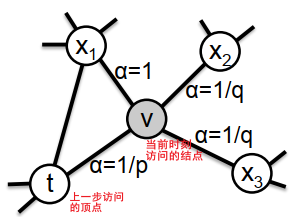
\includegraphics[width=.5\textwidth]{pics/node2vec.png}
	\label{fig:node2vec}
	\caption{Node2Vec中的随机游走}
\end{figure}
Node2vec中的随机游走是二阶的随机游走,为什么叫二阶的呢?在Deepwalk中,随机游走只与当前时刻访问的结点有关,直接从当前节点的邻居中进行均匀采样,这叫一阶。Node2vec中的二阶是指:当前访问的结点$v$,下一步访问的某个节点概率将由上一时刻访问的结点$t$和$v$与邻居的边的权重决定,这是一个二阶马尔科夫链。
$$
P(c_{i}=x \mid c_{i-1}=v)=\left\{\begin{array}{ll}
	\frac{\pi_{v x}}{Z} & \text { if }(v, x) \in E \\
	0 & \text { otherwise }
\end{array}\right.
$$
其中$P(c_{i}=x \mid c_{i-1}=v)$表示当前时刻访问$v$,下一时刻访问$x$的概率,$Z$用于归一化,$\pi_{vx} = \alpha_{pq}(t,x) \cdot w_{vx}$,$\alpha_{pq}(t, x)$为:
$$
\alpha_{p q}(t, x)=\left\{\begin{array}{ll}
	\frac{1}{p} & \text { if } d_{t x}=0 \\
	1 & \text { if } d_{t x}=1 \\
	\frac{1}{q} & \text { if } d_{t x}=2
\end{array}\right.
$$
可见$\alpha_{pq}(t, x)$是一个由$p, q$参数化的函数,函数的自由变量是$t, x$即上一时刻访问的结点和下一时刻访问的结点,其中$d_{tx} \in \{0, 1, 2\}$表示$t, x$间的最短距离。

$p, q$就是控制游走的两个参数:
\begin{itemize}
	\item Return Parameter,$p$,该参数控制下一时刻访问$t$的可能性,如Fig.\ref{fig:node2vec}所示,$p$越小,越有可能访问上一时刻已经访问过的结点$t$,当然还要考虑$w_{vt}$
	\item In-Out Parameter,$q$,该参数能够控制是BFS还是DFS。当$q>1$时,在$p$不变的情况下,访问$d_{tx} = 1$的结点的概率会增大,这就是BFS,当$q<1$时,则会增大访问$d_{tx} = 2$的结点的概率会增大,这就是DFS
\end{itemize}
\begin{figure}[h]
	\centering
	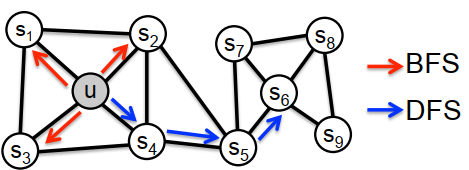
\includegraphics[width=.8\textwidth]{pics/node2vec2.png}
	\label{fig:node2vec2}
	\caption{Homophily与Structure Equivalence}
\end{figure}

论文中将这叫做Biased random walk,通过调整游走的参数$p,q$能够使学习到的表征在同质性(Homophily)和结构相似性(Structure Equivalence)间平衡。BFS能够探索探索homophily,即距离相近的结点,如Fig.\ref{fig:node2vec2}所示,$s_1, s_2, s_3, s_4$是与$u$相邻的结点,它们的表征应该相似;DFS使得探索到更远的地方,能够发现与$u$结构类似地结点,如$s_6$,它俩地表征也应该相似。所以学习到的表征既能体现结点地同质性,也能体现结点地结构相似性。

\subsection{Spectral graph convolution}
谱聚类,主要思想是把所有的数据看做空间中的点,这些点之间可以用边连接起来。距离较远的两个点之间的边权重值较低,而距离较近的两个点之间的边权重值较高,通过对所有数据点组成的图进行切图,让切图后不同的子图间边权重和尽可能的低,而子图内的边权重和尽可能的高,从而达到聚类的目的。

给定一个数据集 $D = \{x_1, x_2, \cdots, x_n\},\ \ x_i \in \mathbb{R}^m$,如何对其进行聚类呢?谱聚类的做法:
\begin{enumerate}
	\item 构建样本之间的相似矩阵;
	\item 根据相似矩阵构建邻接矩阵;
	\item 计算标准化后的拉普拉斯矩阵的特征值和特征向量;
	\item 取最小的 $k1$ 个特征值对应的特征向量,作为原数据集的替代,得到新的特征矩阵;
	\item 对新的特征矩阵进行行归一化;
	\item 在新的特征矩阵的基础上进行聚类。
\end{enumerate}